\chapter{Непрерывное и дискретное преобразование Фурье}
\label{ch:chap1}

\definecolor{codegreen}{rgb}{0,0.6,0}
\definecolor{codegray}{rgb}{0.5,0.5,0.5}
\definecolor{codepurple}{rgb}{0.58,0,0.82}
\definecolor{backcolour}{rgb}{0.95,0.95,0.92}

\lstdefinestyle{mystyle}{
    backgroundcolor=\color{backcolour},   
    commentstyle=\color{codegreen},
    keywordstyle=\color{magenta},
    numberstyle=\tiny\color{codegray},
    stringstyle=\color{codepurple},
    basicstyle=\ttfamily\footnotesize,
    breakatwhitespace=false,         
    breaklines=true,                 
    captionpos=b,                    
    keepspaces=true,                 
    numbers=left,                    
    numbersep=5pt,                  
    showspaces=false,                
    showstringspaces=false,
    showtabs=false,                  
    tabsize=2
}

\lstset{style=mystyle}


\section{Истинный Фурье-образ}

Найдём аналитическое выражение для Фурье-Образа:

$$
\begin{aligned}
    \hat{\prod}(\nu) = \int_{-\infty}^{+\infty}\prod(t)e^{-2\pi i \nu t} dt = \int_{-0.5}^{+0.5}1\cdot e^{-2\pi i \nu t}dt =
    \frac{e^{-2\pi i \nu t}}{-2\pi i \nu}\bigg|_{-0.5}^{+0.5} = \\ \frac{1}{-2\pi i \nu}(e^{-\pi i \nu} - e^{\pi i \nu}) = \frac{sin(\pi \nu)}{\pi \nu} = sinc(\pi \nu)    
\end{aligned}
$$
Тогда графики $\prod(t)$ и $\hat{\prod}(\nu)$ будут выглядеть следующим образом:

\begin{figure}[ht]
    \centering
    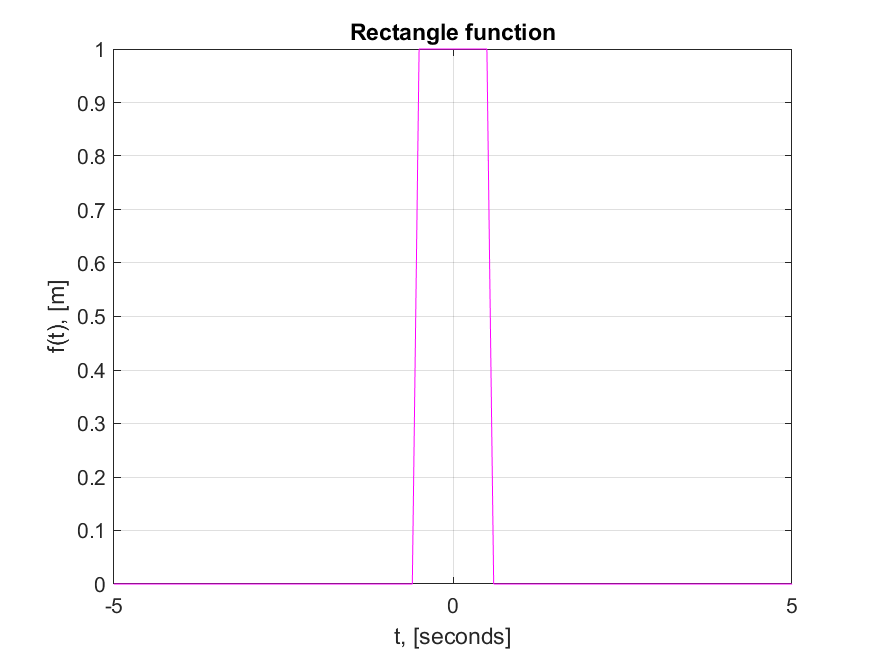
\includegraphics[width=0.7\textwidth]{1_1.png}
	\caption{Прямоугольная функция}
\end{figure}

\begin{figure}[ht]
    \centering
    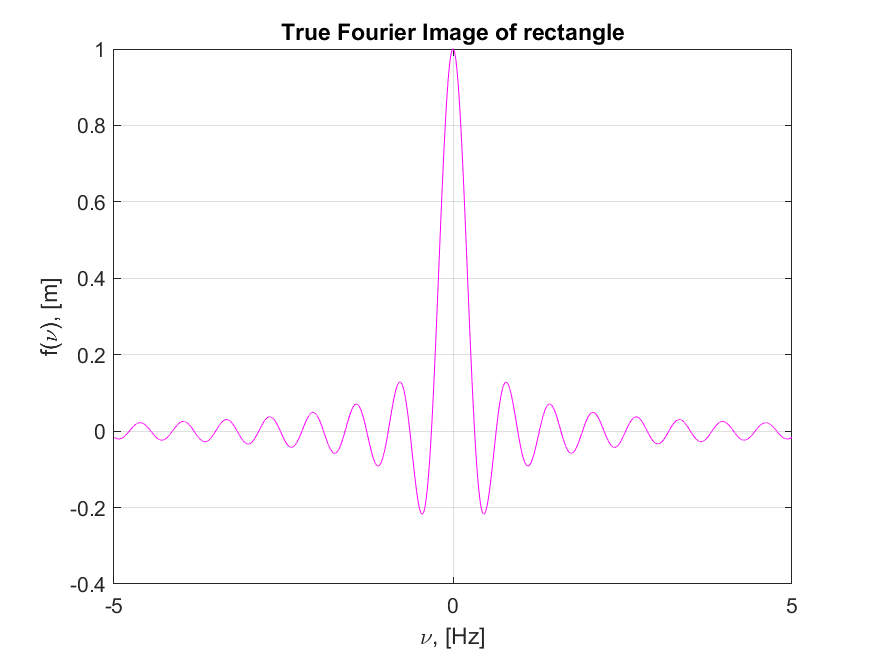
\includegraphics[width=0.7\textwidth]{1_2.png}
	\caption{Фурье-образ прямоугольной функции}
\end{figure}

\section{Численное интегрирование}
$$
\prod(t) \xrightarrow{\texttt{trapz}} \hat{\prod}(\nu) \xrightarrow{\texttt{trapz}} \prod(t)
$$
Теперь будем строить при помощи функции \texttt{trapz} Фурье образы, и сравнивать на то, как они меняются в зависимости от величины шага интегрирования, размера промежутка:

\begin{figure}[!ht]
	\centering
\hspace*{\fill}%
	\begin{subfigure}[b]{0.49\textwidth}
        \centering
		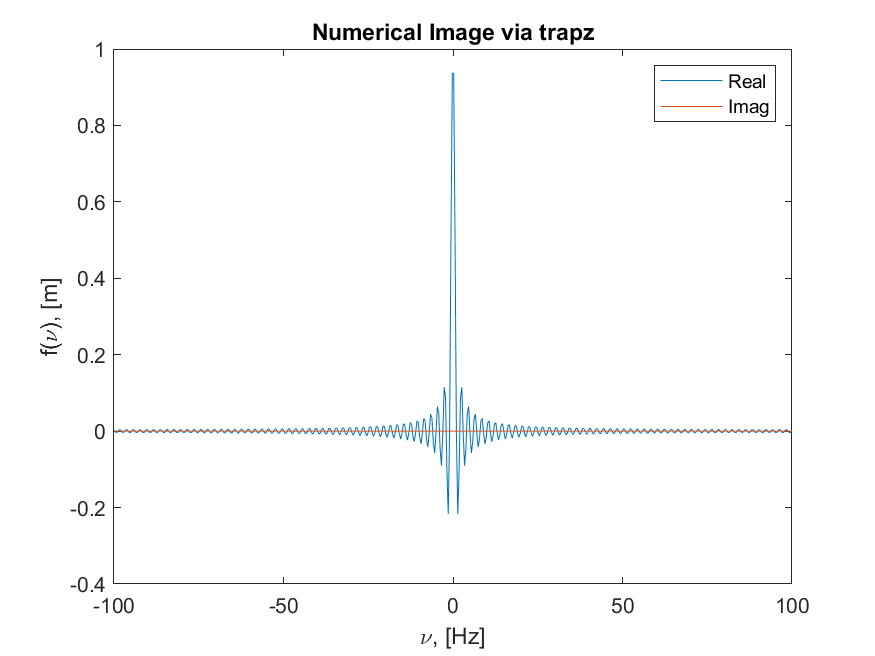
\includegraphics[width=1\textwidth]{1_3.png}
	\end{subfigure}
\hfill
	\begin{subfigure}[b]{0.49\textwidth}
        \centering
		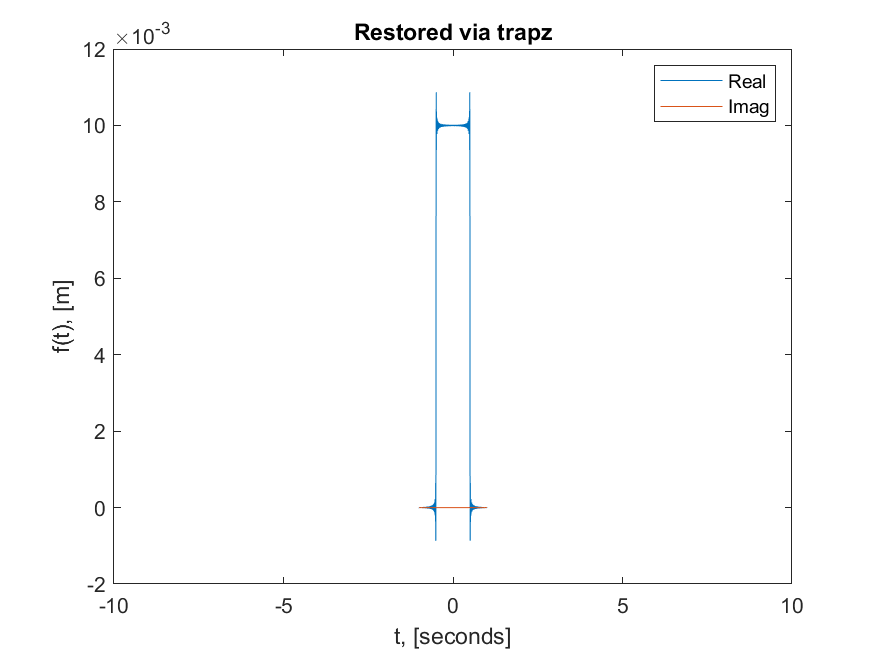
\includegraphics[width=1\textwidth]{1_4.png}
	\end{subfigure}
    \caption{Испытание - Фурье образ и восстановленная функция}
\end{figure}

\newpage

\begin{figure}[!ht]
	\centering
\hspace*{\fill}%
	\begin{subfigure}[b]{0.49\textwidth}
        \centering
		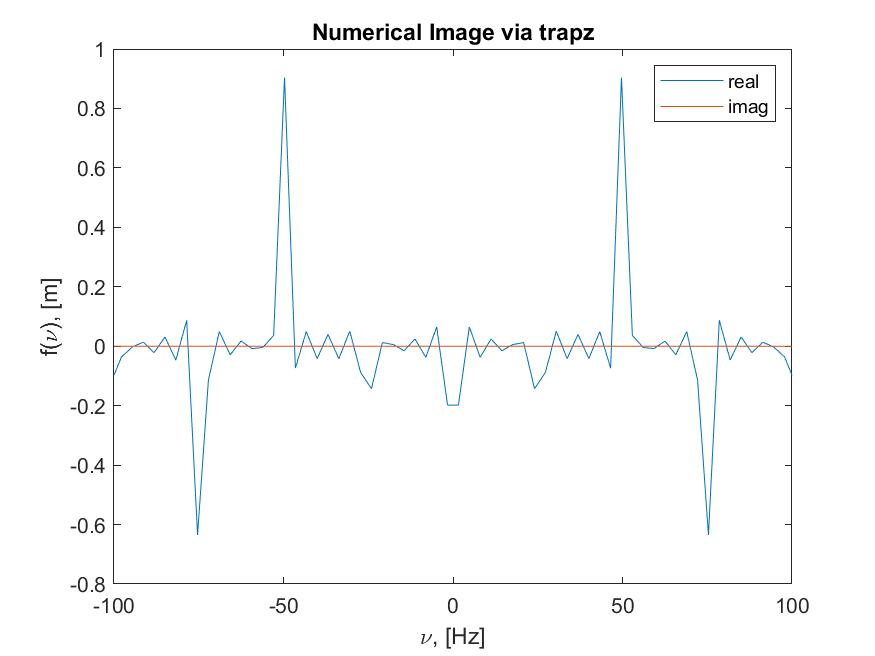
\includegraphics[width=1\textwidth]{1_5.png}
	\end{subfigure}
\hfill
	\begin{subfigure}[b]{0.49\textwidth}
        \centering
		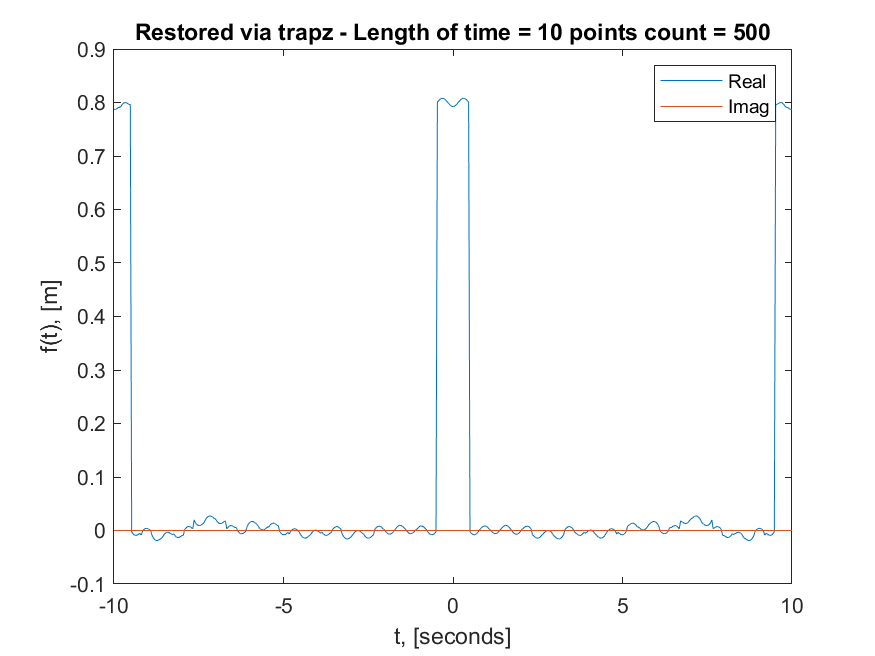
\includegraphics[width=1\textwidth]{1_6.png}
	\end{subfigure}
    \caption{Испытание - Фурье образ и восстановленная функция}
\end{figure}

\begin{figure}[!ht]
	\centering
\hspace*{\fill}%
	\begin{subfigure}[b]{0.49\textwidth}
        \centering
		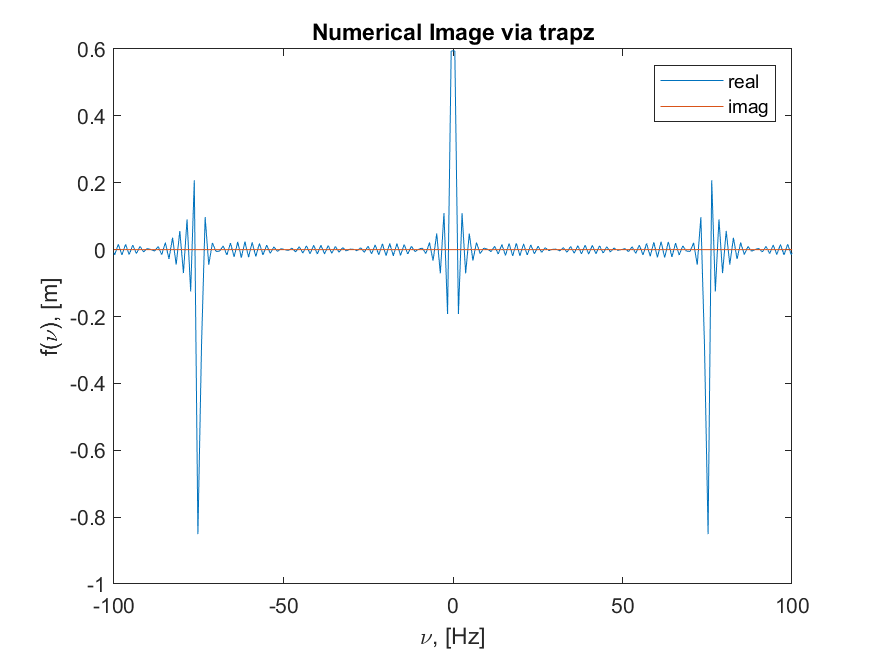
\includegraphics[width=1\textwidth]{1_7.png}
	\end{subfigure}
\hfill
	\begin{subfigure}[b]{0.49\textwidth}
        \centering
		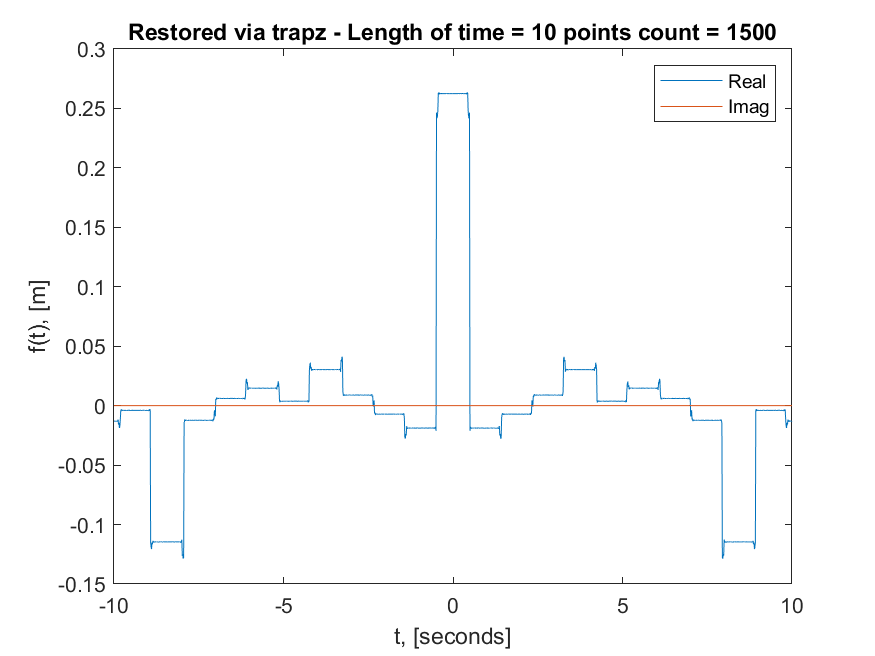
\includegraphics[width=1\textwidth]{1_8.png}
	\end{subfigure}
    \caption{Испытание - Фурье образ и восстановленная функция}
\end{figure}

\newpage
\begin{figure}[!ht]
	\centering
\hspace*{\fill}%
	\begin{subfigure}[b]{0.49\textwidth}
        \centering
		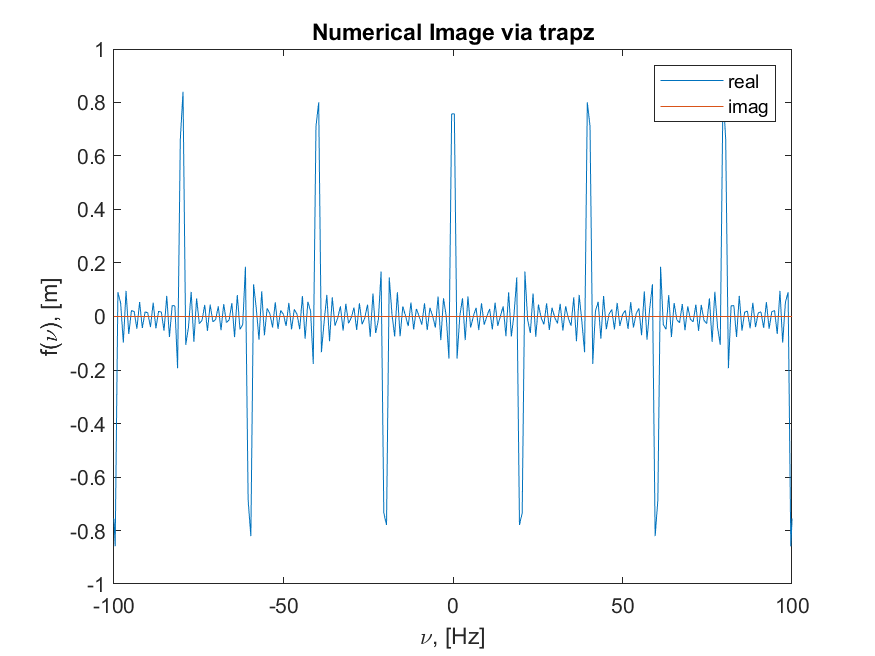
\includegraphics[width=1\textwidth]{1_9.png}
	\end{subfigure}
\hfill
	\begin{subfigure}[b]{0.49\textwidth}
        \centering
		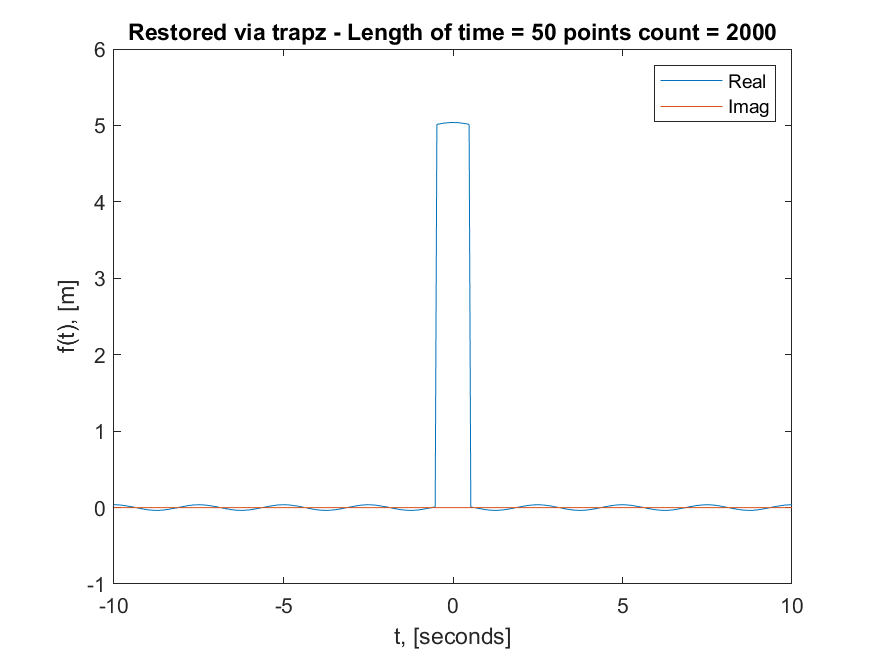
\includegraphics[width=1\textwidth]{1_10.png}
	\end{subfigure}
    \caption{Испытание - Фурье образ и восстановленная функция}
\end{figure}

\begin{figure}[!ht]
	\centering
\hspace*{\fill}%
	\begin{subfigure}[b]{0.49\textwidth}
        \centering
		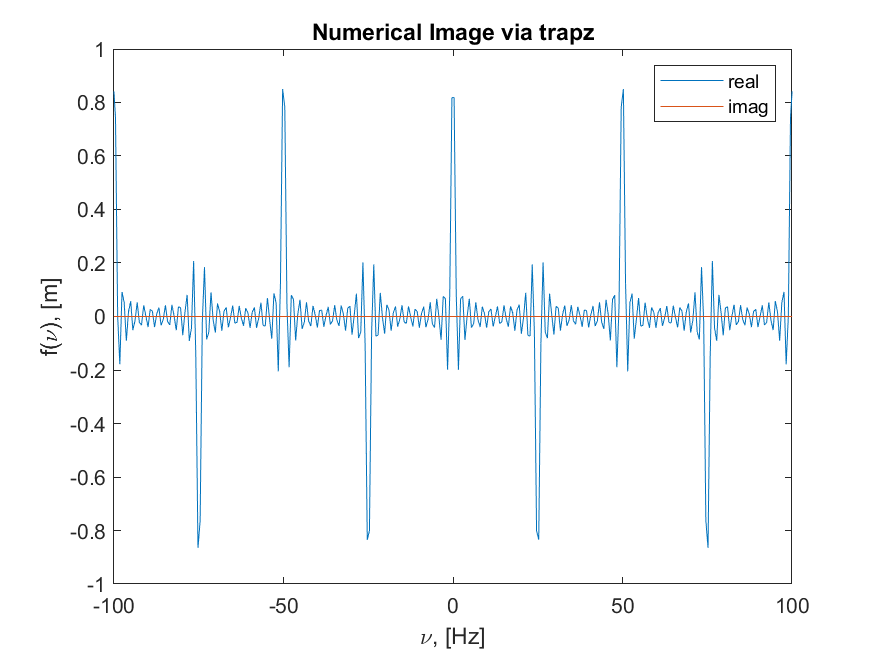
\includegraphics[width=1\textwidth]{1_11.png}
	\end{subfigure}
	\hfill
	\begin{subfigure}[b]{0.49\textwidth}
        \centering
		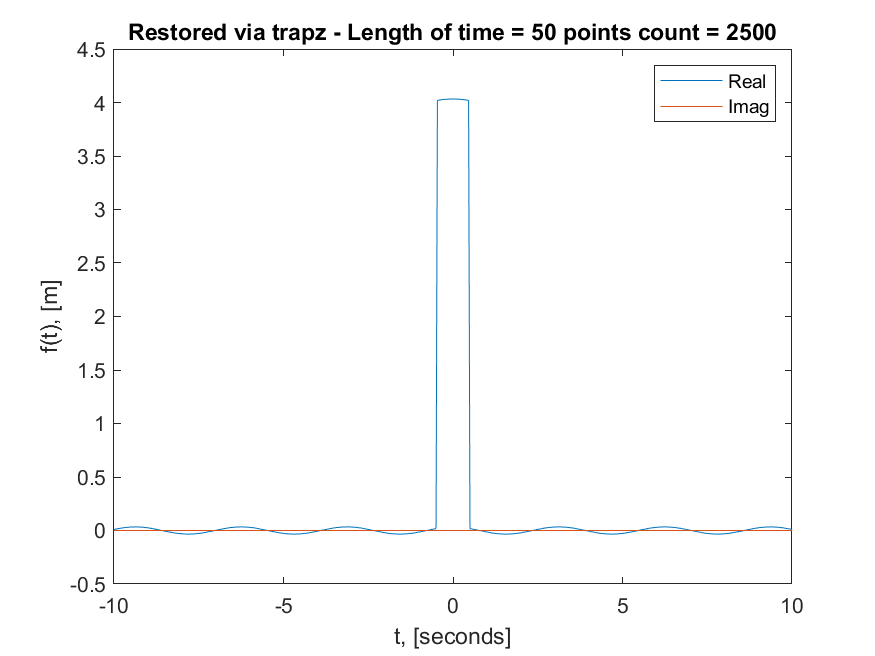
\includegraphics[width=1\textwidth]{1_12.png}
	\end{subfigure}
	\caption{Испытание - Фурье образ и восстановленная функция}
\end{figure}

\begin{figure}[!ht]
	\centering
\hspace*{\fill}%
	\begin{subfigure}[b]{0.49\textwidth}
        \centering
		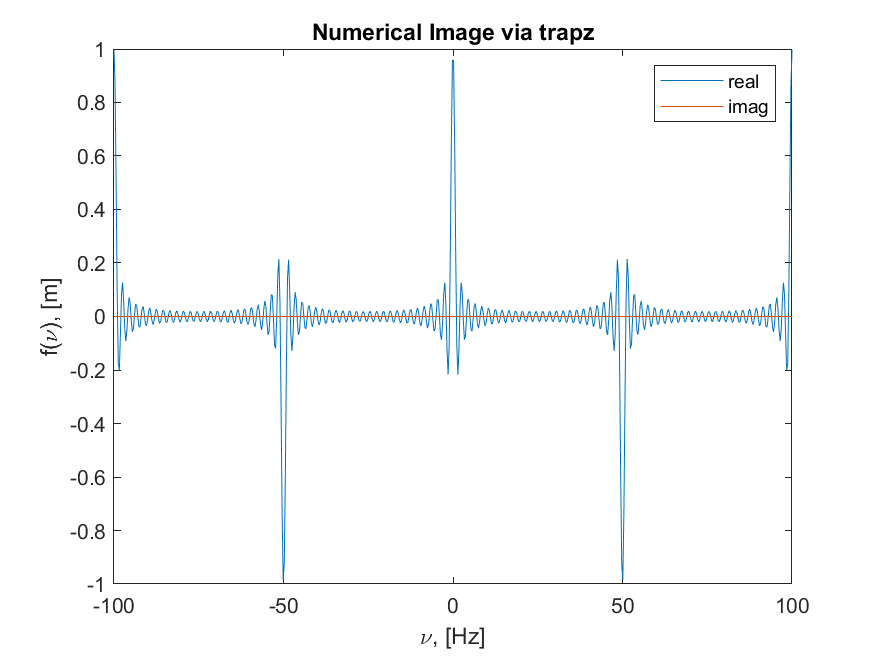
\includegraphics[width=1\textwidth]{1_13.png}
	\end{subfigure}
\hfill
	\begin{subfigure}[b]{0.49\textwidth}
        \centering
		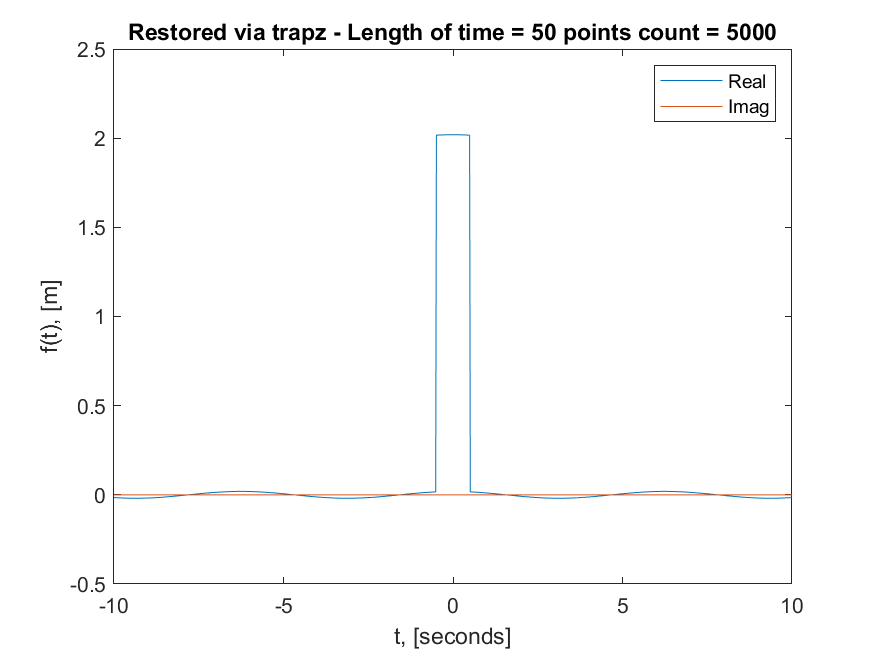
\includegraphics[width=1\textwidth]{1_14.png}
	\end{subfigure}
	\caption{Испытание - Фурье образ и восстановленная функция}
\end{figure}

В итоге мы понимаем, что этот метод уже начнёт нам показывать треугольник при 500+ точек, но мы должны учитывать, что это приближение численными гармониками, также что верхушка прямоугольной функции не сразу станет приближаться к  плоской. 
Поэтому нам удаётся победить периодичность лишь при большом количестве точек(5000+). В итоге - это \textbf{ быстрый способ, но не точный}.

\newpage
\section{Использование DFT}

Найдём Фурье-образ функции $\prod(t)$ с помощью дискретного преобразования Фурье \textit{в унитарной форме}, схематично мы делаем следующее:
$$
\prod(t) \xrightarrow{\texttt{fftshift(fft())}} \hat{\prod}(\nu) \xrightarrow{\texttt{ifft(ifftshift()}} \prod(t)
$$

\begin{figure}[!ht]
	\centering
\hspace*{\fill}%
	\begin{subfigure}[b]{0.49\textwidth}
        \centering
		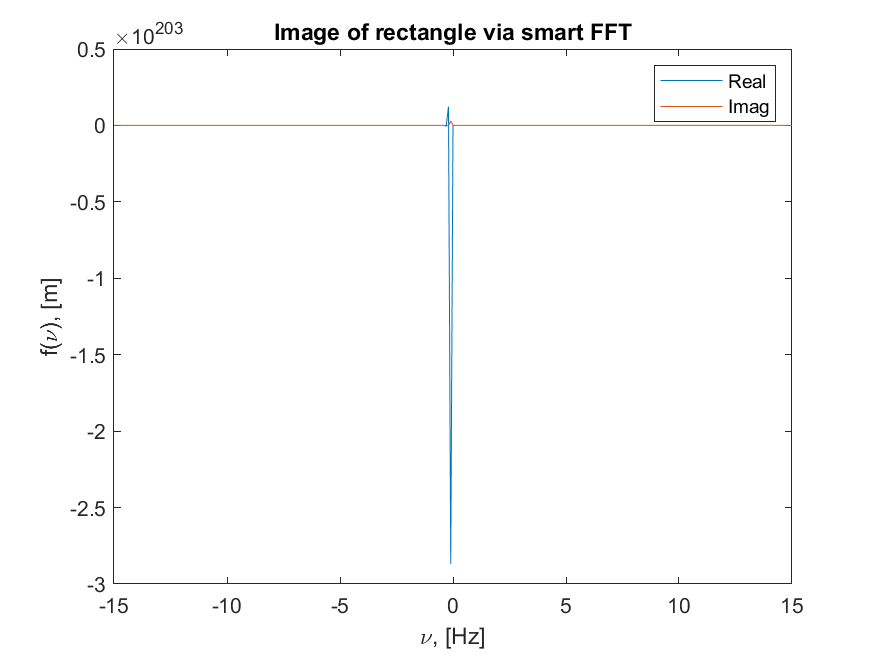
\includegraphics[width=1\textwidth]{1_15.png}
	\end{subfigure}
\hfill
	\begin{subfigure}[b]{0.49\textwidth}
        \centering
		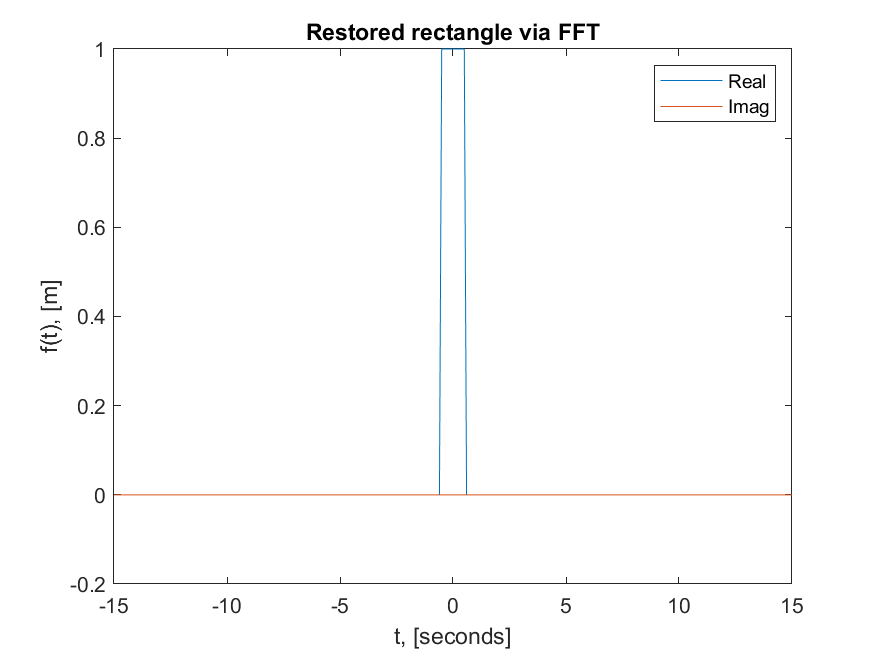
\includegraphics[width=1\textwidth]{1_16.png}
	\end{subfigure}
    \caption{Испытание - Фурье образ и восстановленная функция}
\end{figure}

В итоге мы получили, что восстановленый прямоугольник совпадает с оригинальной функцией (на глаз), но при этом Фурье-образ через \texttt{fft} очень странно выглядит, 
по крайней мере он не похож на другие образы, полученные выше, однако если взять от него модуль, то он уже будет более похож на модули образов выше. 
Думаю, это связано с тем, что такая функция считает образы \textit{более оптимально}, поэтому там и появляются комплексные числа, которых, по идее, не должно быть.

\section{Немного объяснений}

В данном случае оценить скорость работы алгоритмов \texttt{trapz} и \texttt{fft} немного затруднительно, ведь вроде комп не лагал и там и там, а делать целые бенчмарк тесты по заданию вроде не просят.
Но можно понять, что \texttt{trapz} - это всё-таки подобие преобразования Фурье, потому что мы пытаемся численно посчитать интеграл, а это операция более дорогостоящая, чем в случае \texttt{fft} оптимизировать матричное умножение.
Я думаю, как следствие этого, только \texttt{trapz} позволяет нам увидеть адекватный Фурье образ. Касательно обратного преобразования, я думаю здесь ситуация обратная - \texttt{fft} из-за достаточно потери информации благодаря диксретности позволил сделать восстановление идеальным и без эффекта Гиббса в случае \texttt{trapz}.

Основная идея тут: \texttt{trapz} - это всё-таки работа с интегралами, \texttt{fft} - это уже \texttt{DFT}, вектора.

\section{Приближение непрерывного с помощью DFT}

Попробуем исправить ситуацию и совместим достоинства обоих подходов: точность и быстродействие. В этом мне больше всего помогла эта \href{https://medium.com/@alessandrotakeshimorita/actually-computing-fourier-transforms-in-bf1a645a151c}{статья}, если кратко, то мы просто вместо интеграла будем считать римановские суммы, а это уже DFT, которое мы посчитаем с помощью \texttt{fft}.

За основу возьмём формулу унитарного преобразования Фурье через частоты: $\hat{f}(\nu) = \frac{1}{\sqrt{2\pi}}\int_{-\infty}^{+\infty}f(t)e^{-2\pi i \nu t}dt$. Для того, чтобы перейти в \texttt{DFT}, нам нужно дискретизировать эту формулу по временной и частотной оси,
для этого введём следующее: $t_{disc} = t_0 + \alpha\cdot\Delta t$ и $\nu_{disc} = \beta\cdot\Delta\nu$ , где $\alpha \in[0,\dots,N-1]$. Также подметим, что интеграл будет по левым суммам, и количество точек в 
исходной последовательности определяется следующим соотношением $\Delta\nu = \frac{1}{N\Delta t}$, где $N$ - количество точек в исходной последовательности, тогда:

$$
\begin{aligned}
	\hat{f}(\nu) = \frac{1}{\sqrt{N}}\sum_{\alpha=0}^{N-1}f(t_{disc})e^{-2\pi i \nu t}\Delta t = \frac{1}{\sqrt{N}}\sum_{\alpha=0}^{N-1}f(t_0 + \alpha\Delta t)e^{-2\pi i \nu (t_0 + \alpha\Delta t)}\Delta t = \\
	\Delta t e^{-2\pi i \nu t_0}\frac{1}{\sqrt{N}}\sum_{\alpha=0}^{N-1}f(t_0 + \alpha\Delta t)e^{-2\pi i \nu \alpha\Delta t}
\end{aligned}
$$
А теперь добавим дискретизированные частоты:
$$
\begin{aligned}
	\hat{f}(\nu_{disc}) = \Delta t e^{-2\pi i \nu_{disc} t_0}\frac{1}{\sqrt{N}}\sum_{\alpha=0}^{N-1}f(t_0 + \alpha\Delta t)e^{-2\pi i \Delta\nu \alpha\Delta t} = \\
	\Delta t e^{-2\pi i \nu_{disc} t_0}\frac{1}{\sqrt{N}}\sum_{\alpha=0}^{N-1}f(t_0 + \alpha\Delta t)e^{-2\pi i \alpha / N} = \Delta t e^{-2\pi i \nu_{disc} t_0} \mathbb{F}\{f(t_{disc})\}
\end{aligned}
$$
В последнем равенстве мы заменили громоздкое суммирование на один единственный оператор - \texttt{DFT}. Получается, что мы можем получить образ Фурье из функции через \texttt{DFT}, если умножим его на \textit{коэффициент}, похожий на сдвиг.

Для обратного преобразование проведём аналогичные рассуждения, для начала запишем:
$$
f(t) = \frac{1}{\sqrt{2\pi}}\int_{-\infty}^{+\infty}\hat{f}(\nu)e^{2\pi i \nu t}d\nu
$$, из чего получим\dots
$$
f(t_{disc}) = \frac{1}{\sqrt{N}}\sum_{\beta = 0}^{N-1}\hat{f}(\nu_{disc})e^{2\pi i \beta \Delta\nu \alpha \Delta t}\Delta\nu = \Delta\nu\mathbb{F}\{\hat{f}(\nu_{disc})\}
$$

В итоге и обратное преобразование Фурье требует только домножения на коэффициент, в итоге вот так выглядит наш успех:
$$
\prod(t) \xrightarrow{Smart::\texttt{FFT}} \hat{\prod}(\nu) \xrightarrow{Smart::\texttt{iFFT}} \prod(t)
$$

Где за $t_0$ мы просто берём начало вектора времени. Проверим на практике полученные формулы:

Почему-то мне так и не удалось получить красивые-верные практические результаты, я остановился примерно на этом:

\begin{figure}[!ht]
	\centering
\hspace*{\fill}%
	\begin{subfigure}[b]{0.49\textwidth}
        \centering
		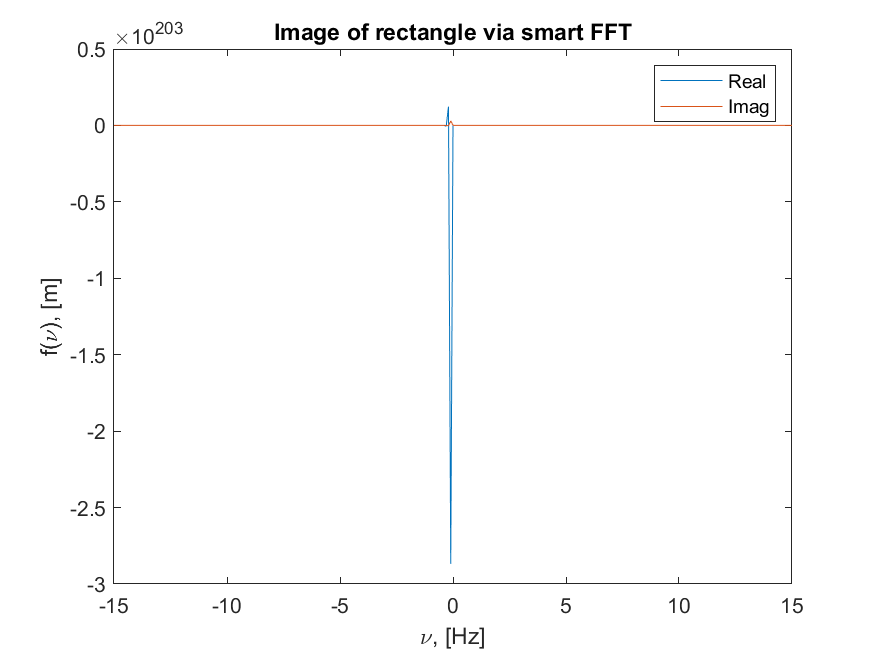
\includegraphics[width=1\textwidth]{1_17.png}
	\end{subfigure}
\hfill
	\begin{subfigure}[b]{0.49\textwidth}
        \centering
		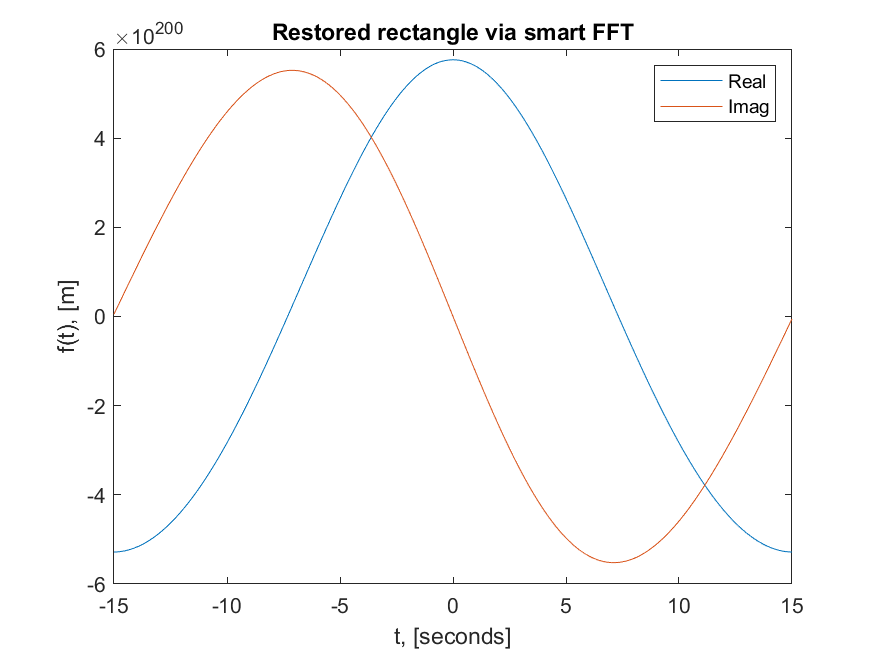
\includegraphics[width=1\textwidth]{1_18.png}
	\end{subfigure}
    \caption{Неудача при использовании Smart FFT}
\end{figure}

\textit{Грустно, но что поделать :(}

\endinput